%%%%%%%%%%%%%%%%%%%%%%%%%%%%%%%%%%%%%%%%%
% Dreuw & Deselaer's Poster
% LaTeX Template
% Version 2.0 (February 18, 2023)
%
% This template originates from:
% https://www.LaTeXTemplates.com
%
% Authors:
% Vel (vel@latextemplates.com)
% Philippe Dreuw and Thomas Deselaers (https://github.com/deselaers/latex-beamerposter)
%
% License:
% CC BY-NC-SA 4.0 (https://creativecommons.org/licenses/by-nc-sa/4.0/)
%
% NOTE: The bibliography needs to be compiled using the bibtex engine.
%
%%%%%%%%%%%%%%%%%%%%%%%%%%%%%%%%%%%%%%%%%

%----------------------------------------------------------------------------------------
%	PACKAGES AND OTHER DOCUMENT CONFIGURATIONS
%----------------------------------------------------------------------------------------

\documentclass{beamer} % Use the beamer base class

\usepackage[
	orientation=portrait, % Portrait orientation
	size=a0, % Paper size
	scale=1.23, % Scale, it's important to adjust this so your content fits nicely in the template
]{beamerposter} % Use the beamerposter package to create the layout

\usetheme{I6pd2} % Use the I6pd2 theme supplied with this template

\def\E{\mathbb{E}} % Expectation symbol
\newcommand{\x}{\textbf{v}}

\usepackage{changepage} % Required for temporarily indenting text blocks

\usepackage{graphicx}

\usepackage{amsmath,amsthm,amssymb,latexsym} % For including math equations, theorems, symbols, etc

\usepackage{gfsdidot} % Use the GFS Didot font

\usepackage{booktabs} % Top and bottom rules for tables

\graphicspath{{Figures/}} % Location of figure images

%----------------------------------------------------------------------------------------
%	TITLE SECTION
%----------------------------------------------------------------------------------------

\title{\LARGE Volatility Forecasting Using Similarity-based Parameter Correction and Aggregated Shock Information} % Poster title

\author{David P. Lundquist\textsuperscript{1} and Daniel J. Eck\textsuperscript{1}} % Author(s)

\institute{\textsuperscript{1}Department of Statistics, University of Illinois Urbana-Champaign} % Institution(s)

%----------------------------------------------------------------------------------------
%	FOOTER TEXT
%----------------------------------------------------------------------------------------

\newcommand{\leftfoot}{https://www.LaTeXTemplates.com} % Left footer text

\newcommand{\rightfoot}{john@latextemplates.com} % Right footer text

\setbeamertemplate{footline}{} % Uncomment this line to hide the footer

%----------------------------------------------------------------------------------------

\begin{document}

\begin{frame}[t] % The whole poster is enclosed in one beamer frame, the [t] parameter aligns everything to the top

\begin{columns}[t] % Begin multi-column layout, the [t] parameter aligns each column's content to the top

\begin{column}{0.02\textwidth}\end{column} % Empty column for horizontal whitespace

\begin{column}{0.465\textwidth} % Start the first content column

%----------------------------------------------------------------------------------------
%	OBJECTIVES
%----------------------------------------------------------------------------------------

\begin{block}{Introduction - Reacting to the Unprecedented}
	\begin{enumerate}
		\item Reacting to a seemingly unprecedented event might involve the question: what, if anything, does it resemble from the past? 
		\begin{figure}
			
\includegraphics[scale = .6]{../NYS_state.png}
		\end{figure} 
		\item Matching a crisis to past events is a problem with unsurprising statistical angles: identification, sample size, weighting, risk, robustness.
		\item Here we employ a method to improve our GARCH-X volatility forecasts under unprecedented conditions.
	\end{enumerate}


\end{block}

%----------------------------------------------------------------------------------------
%	INTRODUCTION
%----------------------------------------------------------------------------------------
            
\begin{block}{The Family of GARCH-X Volatility Models}
	We define a family of $n+1$ univariate times series, each of length $T_{i}$, $i=1,...n+1$.  For each $i$, there exists a news shock that occurs strictly between $T^{*}_{i}$ and $T^{*}_{i}+1$, and for each $i$, there exists a GARCH-X model

	\bigskip % Vertical whitespace


		% $\sigma_{t}^{2} = \omega+ \sum^{m}_{k=1}\alpha_{k}a^{2}_{t-k} + \sum_{j=1}^{s}\beta_{j}\sigma_{t-j}^{2} + \gamma^{T}\x_{t} \text{ .}\label{GARCH-X}$


			  \begin{equation} \sigma^{2}_{i,t} = \omega_{i} + \sum^{m_{i}}_{k=1}\alpha_{i,k}a^{2}_{i,t-k} + \sum_{j=1}^{s_{i}}\beta_{i,j}\sigma_{i,t-j}^{2} + \gamma_{i}^{T} \x_{i,t} + \omega^{*}_{i,t}
			  \end{equation}
		  
			  \begin{equation}a_{i,t} = \sigma_{i,t}\epsilon_{i,t} 
			  \end{equation}

with the ``unprecedented" shocks parameterized by

\begin{equation}\omega_{i,t}^{*} = D^{vol}_{i,t}[\mu_{\omega^{*}}+\delta^{T}\x_{i,T^{*}_{i}+1}+ u_{i,t}]
\end{equation}

where $\x_{i,T^{*}_{i}+1}$ is a vector of variables, deterministic with respect to $\mathcal{F}_{T^{*}_{i}+1}$, that reflects and encodes prevailing risk conditions.  All other errors are mean-zero and idiosyncratic.


	\end{block}



%----------------------------------------------------------------------------------------
%	MATERIALS
%----------------------------------------------------------------------------------------
\begin{block}{Objective}
Provide a one-step-ahead volatility forecast for the \textit{time series under study}, i.e. the first time series in the family above.  We will denote the series $i=2,...,n+1$ the \textit{donor series}, from which we will extract information.
\end{block}

\begin{block}{Forecast Methodology}
We estimate the "unprecedented" shocks in the donor pool (i.e., $i = 2,3,...n+1$) using fixed-effect estimation during the shock times, yielding shock estimators $\{\hat\omega_{i,*}\}_{i=2}^{n+1}$.  The aggregated shock estimator is given by

\begin{equation}
	\hat\omega^{*} = \sum^{n+1}_{i=2}\pi_{i}\hat\omega^{*}_{i,*}
\end{equation}

where the weights $\{\pi_{i}\}_{i=2}^{n+1}$ are non-negative, sum to one, and chosen to minimize the $L^{2}$-norm of the difference of $\x_{i,T^{*}_{i}}$ and the convex hull of $\{\x_{i,T^{*}_{i}}\}^{n+1}_{i=2}$, similar to the Synthetic Control approach in causal inference \cite{abadie2003economic,abadie2010synthetic}.  We then produce an adjusted one-step-ahead forecast of the time series under study:

%The weights $\{\pi{i}\}_{i=2}^{n+1}$ help us to build a `clone' of the shock that will hit the time series under study.

\begin{equation}
	\hat\sigma^{2}_{1,t+1} = \hat\omega_{1} + \sum^{m_{1}}_{k=1}\hat\alpha_{1,k}a^{2}_{1,t+1-k} + \sum_{j=1}^{s_{1}}\hat\beta_{1,j}\sigma_{1,t+1-j}^{2} + \hat\gamma_{1}^{T} \x_{1,t+1} + \textcolor{red}{\hat\omega^{*}}
\end{equation}

\end{block}

%----------------------------------------------------------------------------------------
%	METHODS
%----------------------------------------------------------------------------------------

\begin{block}{Evaluating Forecasts with QL Loss}
	
\begin{equation}
\text{QL}^{h}_{method, ground truth} = \frac{\hat\sigma^{2}_{h, ground truth}}{ \hat\sigma^{2}_{h, method}} - \log{\frac{\hat\sigma^{2}_{h, ground truth}}{ \hat\sigma^{2}_{h, method}}} -1 
\end{equation}




	\begin{itemize}
		\item Quasi-likelihood Loss is that it is multiplicative rather than additive.
		\item The technical properties of the QL Loss allow researchers to compare forecasts across heterogeneous time series, whereas additive loss functions like MSE unfairly penalize forecasts made under market turbulence \cite{brownlees2011practical}.

	\end{itemize}
\end{block}

\end{column} % End of the first column



\begin{column}{0.03\textwidth}\end{column} % Empty column for horizontal whitespace
 
\begin{column}{0.465\textwidth} % Start the second content column

%----------------------------------------------------------------------------------------
%	RESULTS
%----------------------------------------------------------------------------------------

	
    % \begin{figure}[!h]
	% 	\centering
	% 	\textbf{Signal and Noise}\par\medskip
	%   \begin{subfigure}{.44\linewidth} 
	% 	\centering
	% 	  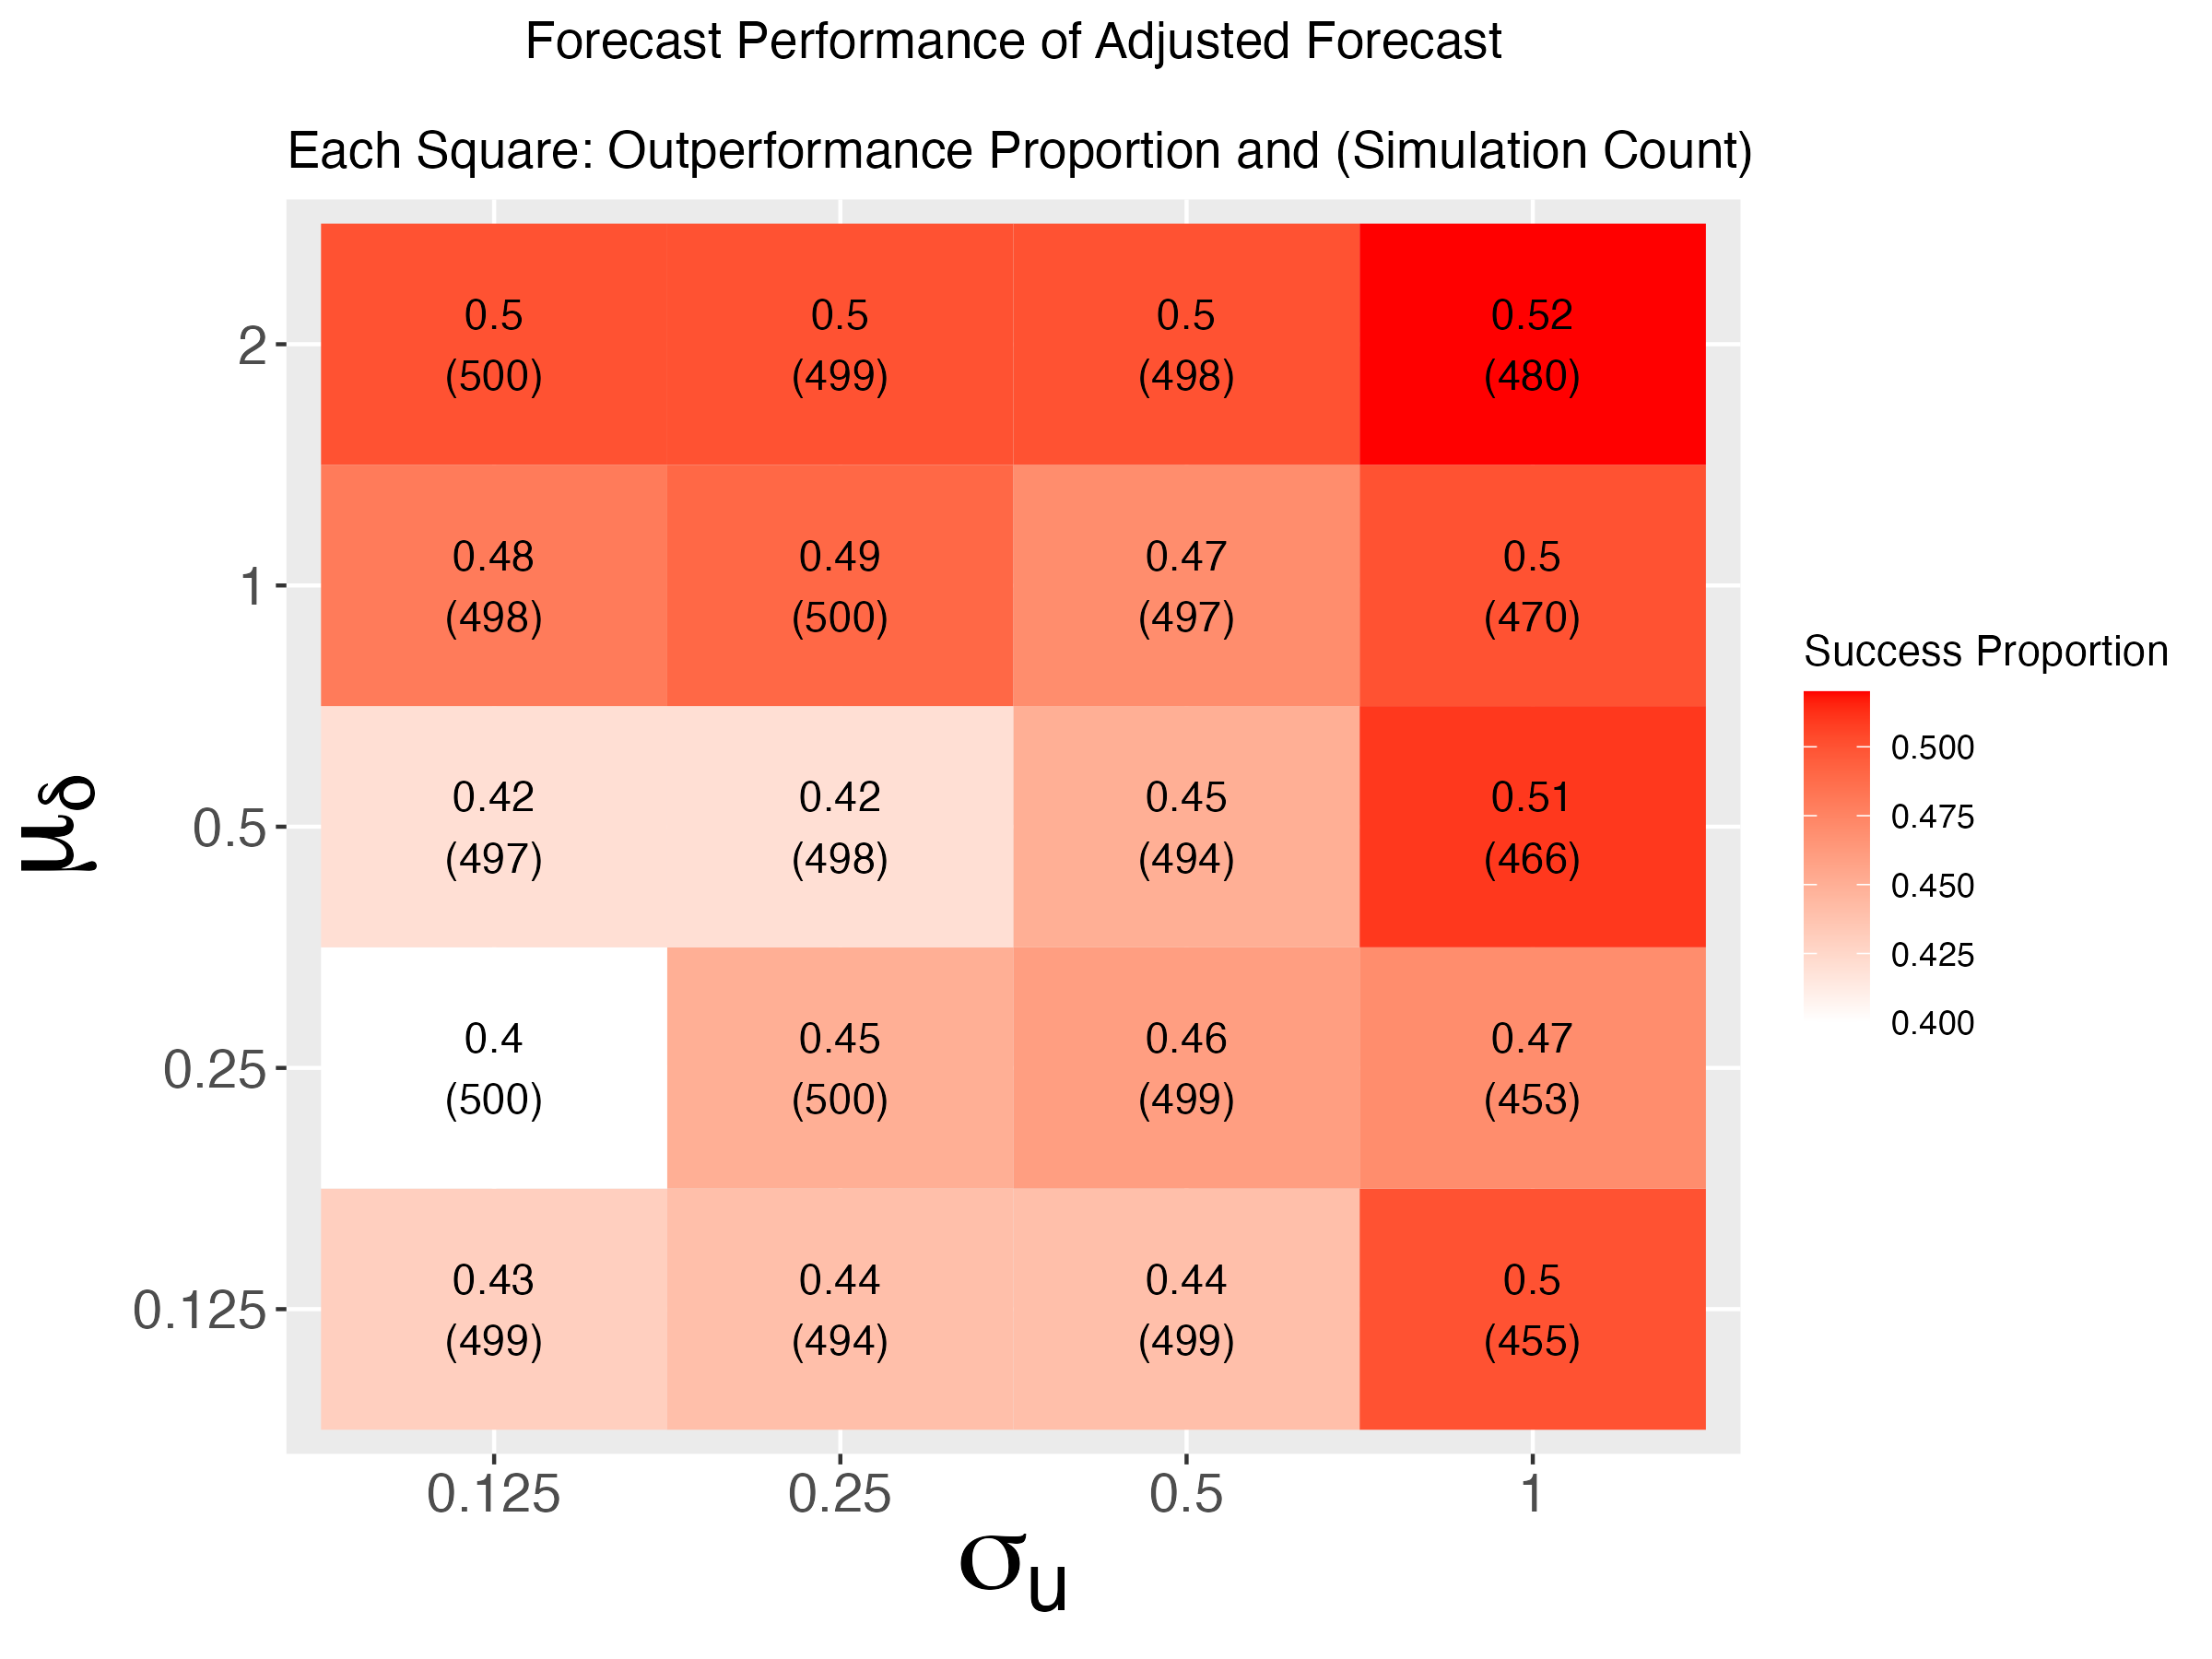
\includegraphics[scale = .42]{../simulation_plots/Aug28_224311_2024_mu[delta]_sigma[u].png}
	% 	  \caption{Fixed values: $\mu_{v} = .125, \sigma_{v} = .125, \mu_{\omega^{*}} = .125$}\label{fig:sim_1}
	%   \end{subfigure}\hspace{12mm} %
	%   \begin{subfigure}{.44\linewidth} 
	% 	\centering
	% 	  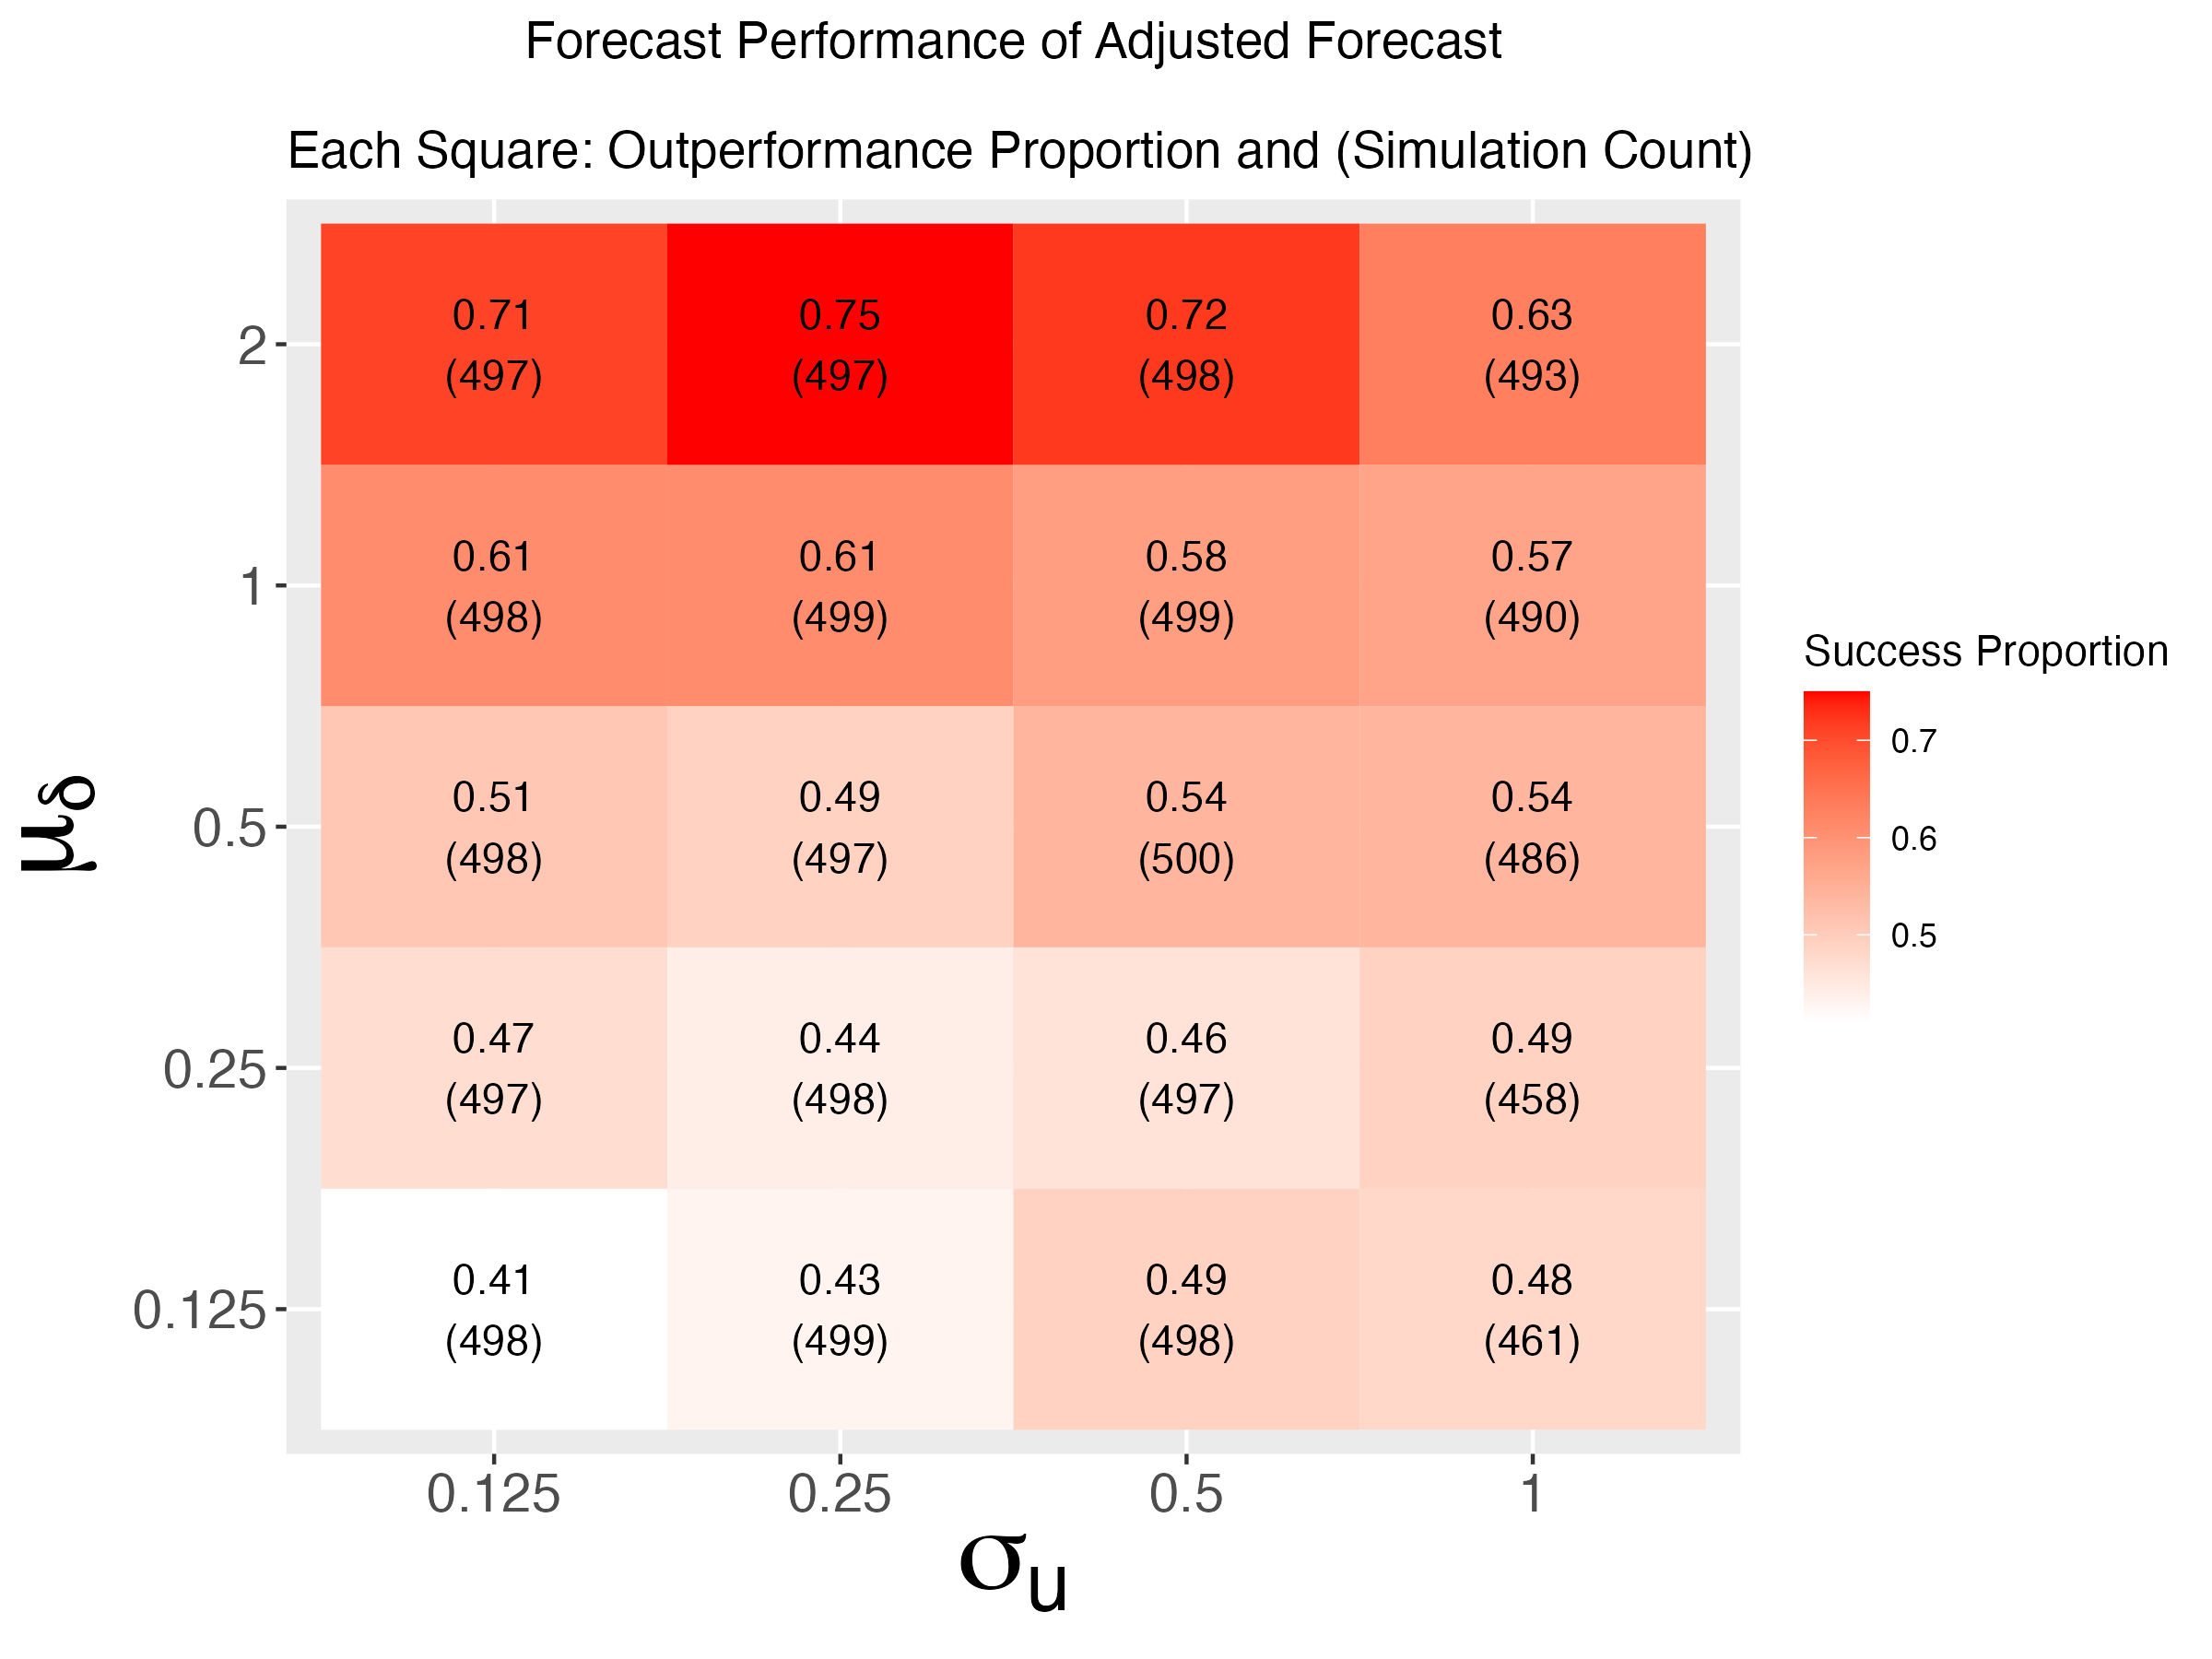
\includegraphics[scale=.42]{../simulation_plots/Aug28_224317_2024_mu[delta]_sigma[u].png}
	% 	  \caption{Fixed values: $\mu_{v} = .5, \sigma_{v} = .125, \mu_{\omega^{*}} = .125$}\label{fig:sim_2}
	%   \end{subfigure}
  
	%   \begin{subfigure}{.44\linewidth} 
	% 	\centering
	% 	  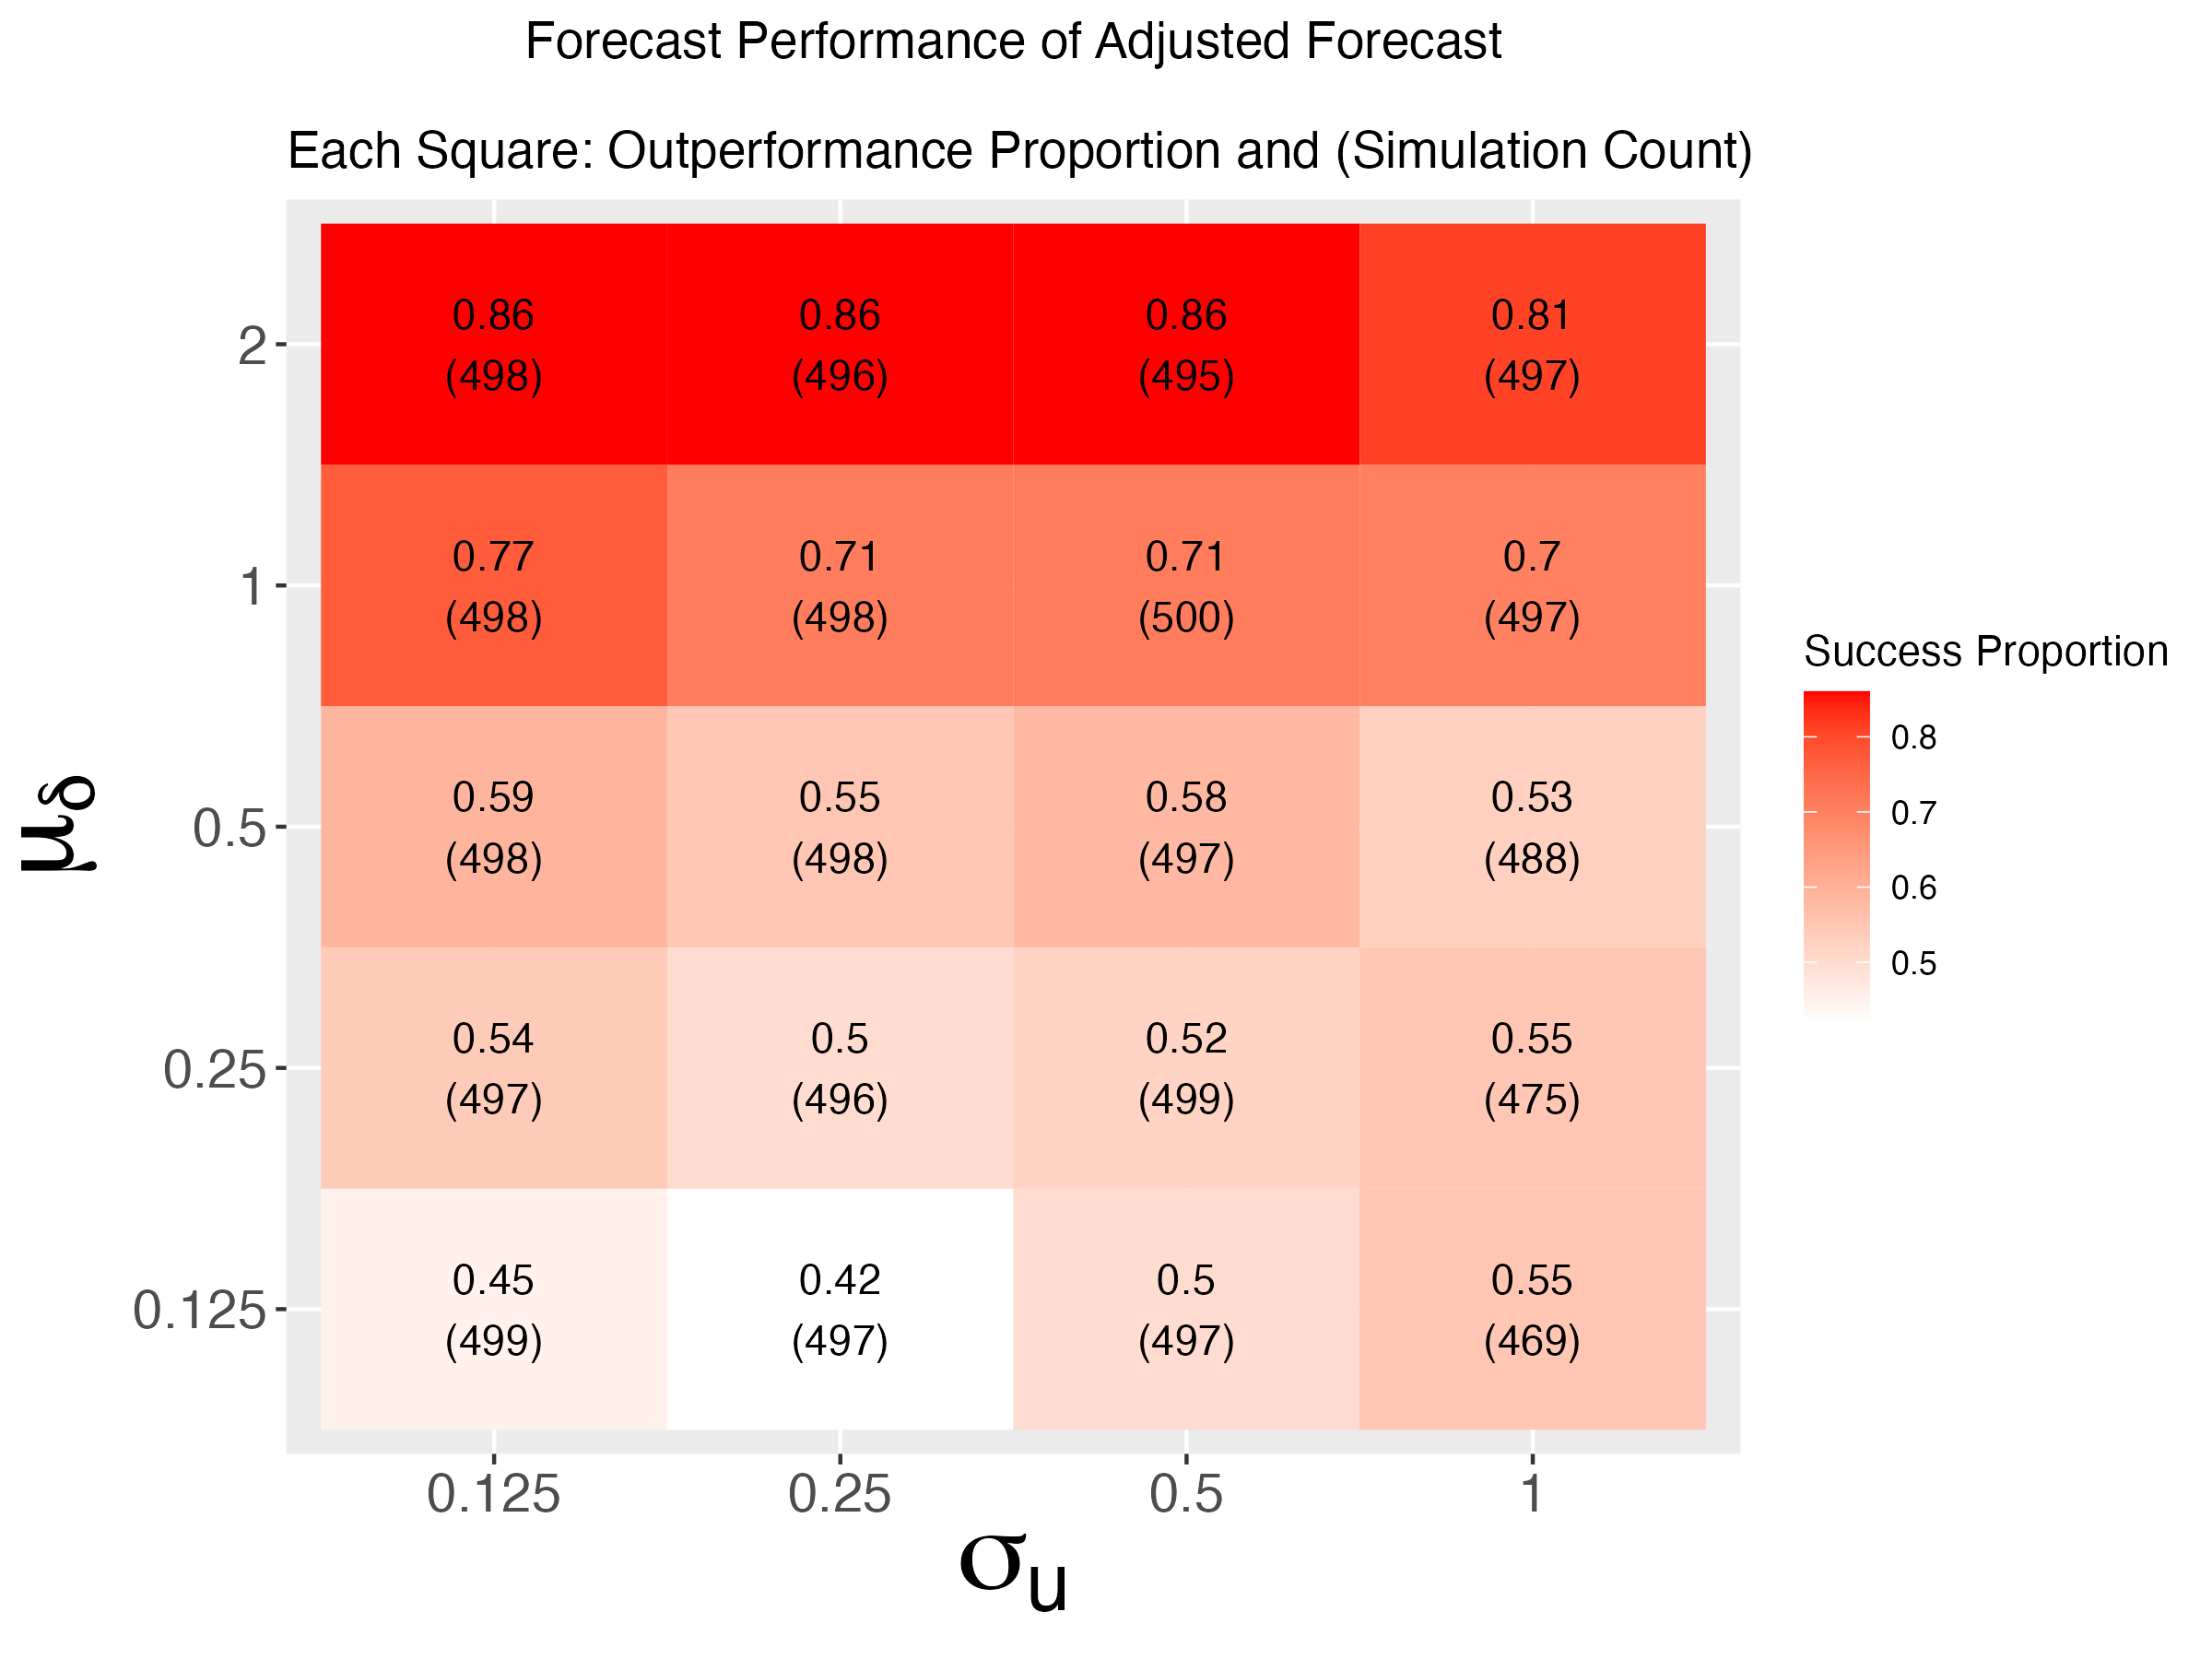
\includegraphics[scale=.42]{../simulation_plots/Aug28_224322_2024_mu[delta]_sigma[u].png}
	% 	  \caption{Fixed values: $\mu_{v} = 1, \sigma_{v} = .125, \mu_{\omega^{*}} = .125$}\label{fig:sim_3}
	%   \end{subfigure}
	  
	% 	  \caption{In the progression from \ref{fig:sim_1} to \ref{fig:sim_2} to \ref{fig:sim_3}, we see that increasing $\mu_{\delta}$ leads to improved performance of the adjusted forecast, and this effect is intensified as $\mu_{v}$ increases.  However, it is not consistently true that an increasing noise undermines the performance of the adjusted forecast.  Rather, that phenomenon requires both large quantites of $\mu_{\delta}$ and $\mu_{v}$.}
	% 	  \label{fig:signoise}
	% 	\end{figure}
  
% 	\begin{figure}[!h]
% 	  \centering
% 	  \textbf{Interaction between Signal and Volatility Profile Means}\par\medskip
% 	\begin{subfigure}{.44\linewidth} 
% 	  \centering
% 		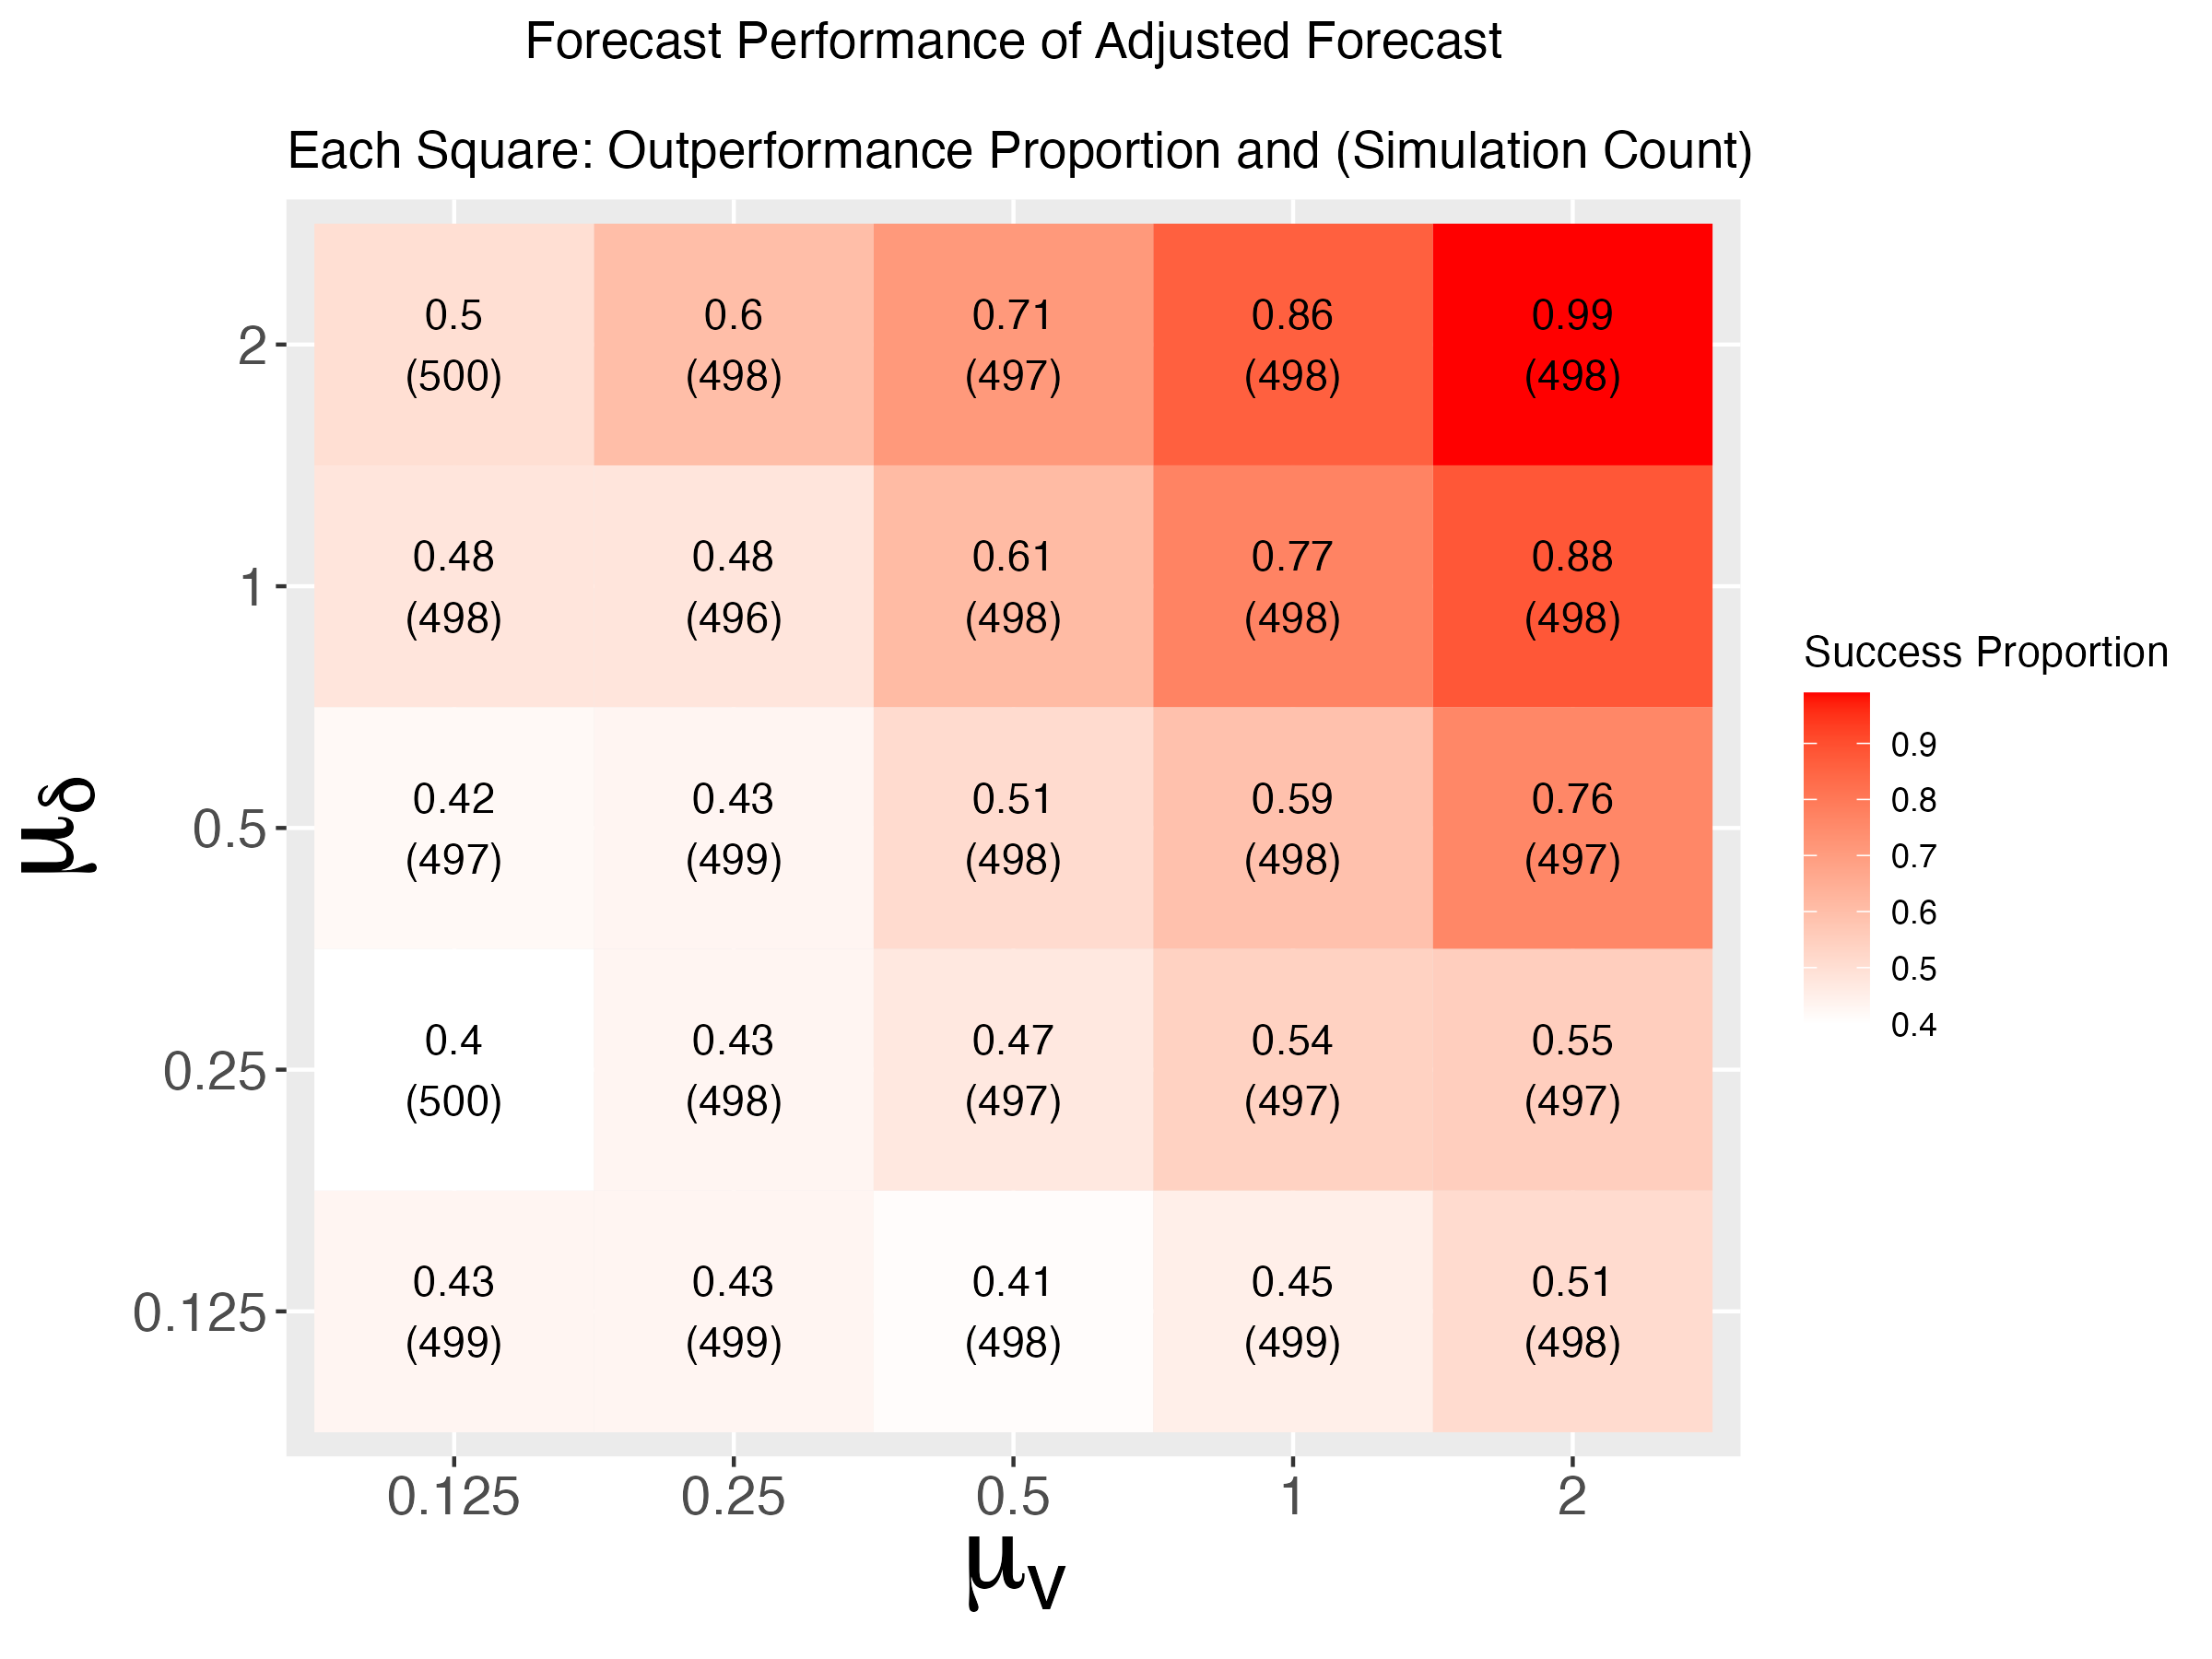
\includegraphics[scale = .42]{simulation_plots/Aug28_224330_2024_mu[delta]_mu[v].png}
% 		\caption{Fixed values: $\sigma_{v} = .125, \mu_{\omega^{*}} = .125, \sigma_{u} = .125$}\label{fig:sim_4}
% 	\end{subfigure}\hspace{12mm} %
% 	\begin{subfigure}{.44\linewidth} 
% 	  \centering
% 		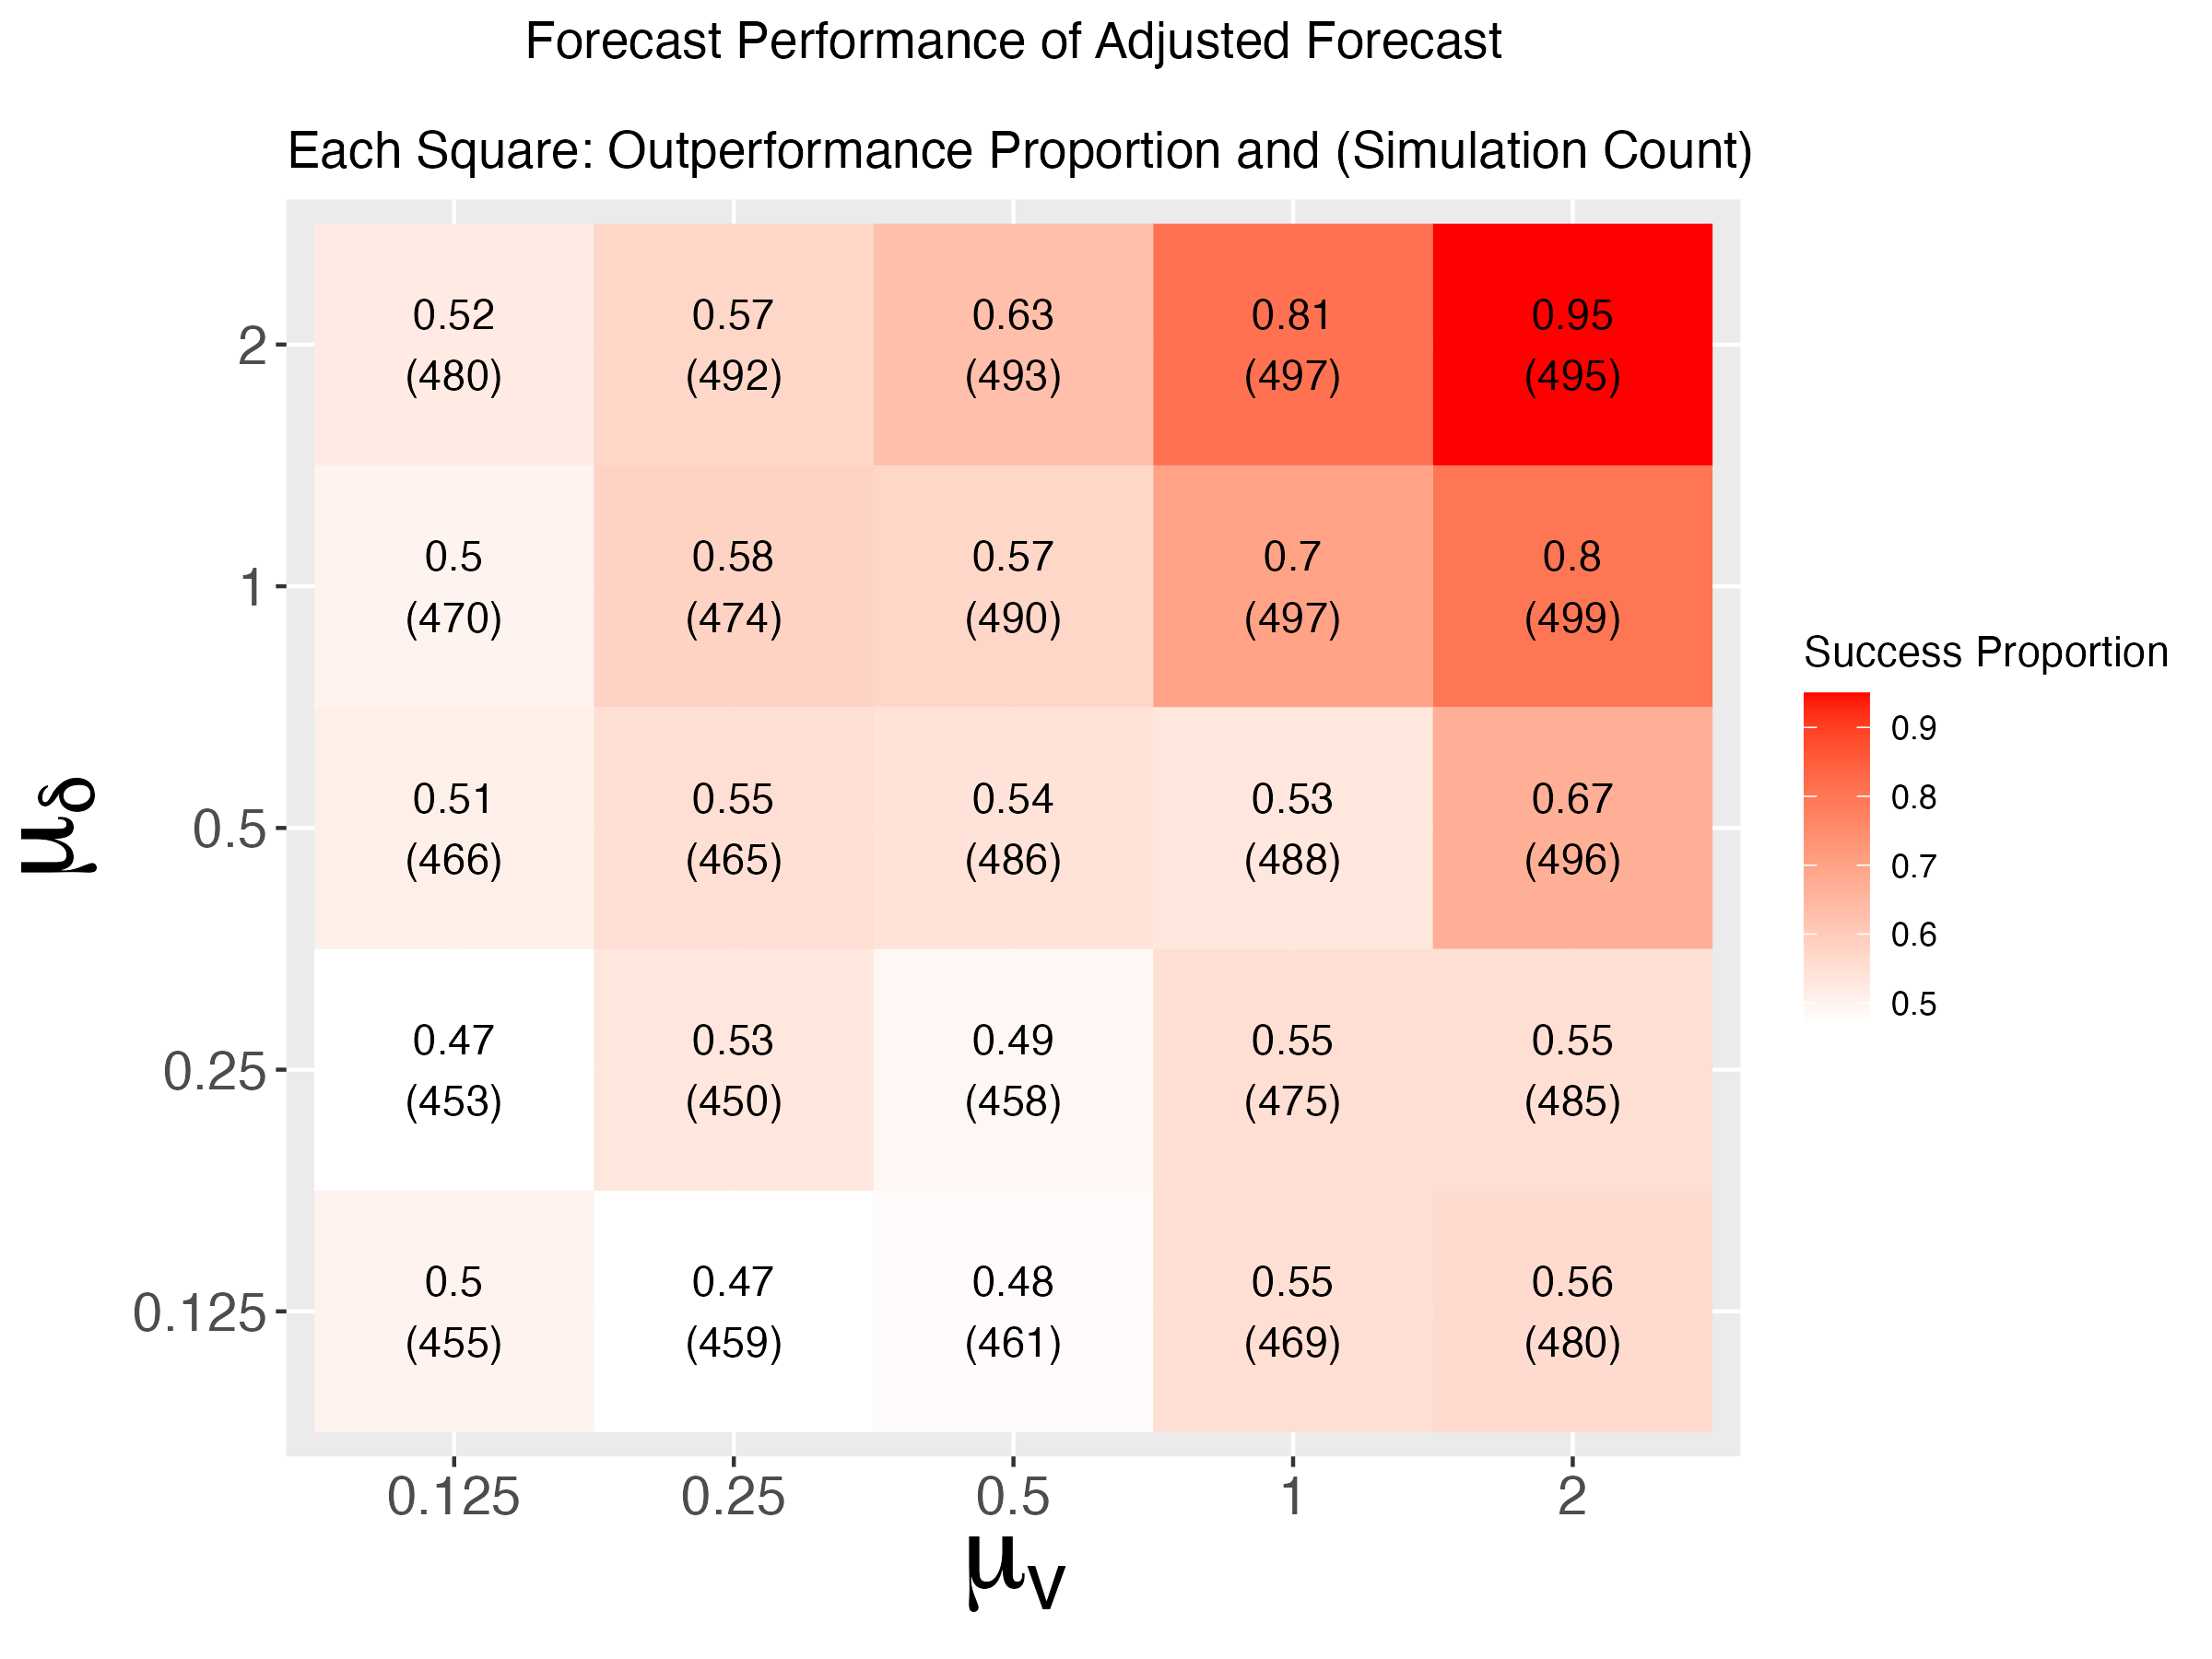
\includegraphics[scale=.42]{simulation_plots/Aug28_224337_2024_mu[delta]_mu[v].png}
% 		\caption{Fixed values: $\sigma_{v} = .125, \mu_{\omega^{*}} = .125, \sigma_{u} = 1$}\label{fig:sim_5}
% 	\end{subfigure}
	
% 		\caption{We compare the interaction of $\mu_{\delta}$ and $\mu_{v}$ at two different levels of shock noise.  In the low-noise regime, the peak performance of the adjusted forecast is higher, and the ascent is faster along both dimensions.   However, in the high-noise regime, the adjusted forecast performs well even at low levels of $\mu_{\delta}$ and $\mu_{v}$.}
% 		\label{fig:sig_volprof}
% 	  \end{figure}
  
%   \begin{figure}[!h]
% 	\centering
% 	\textbf{Interaction between Shock Intercept and Shock Noise}\par\medskip
%   \begin{subfigure}{.44\linewidth} 
% 	\centering
% 	  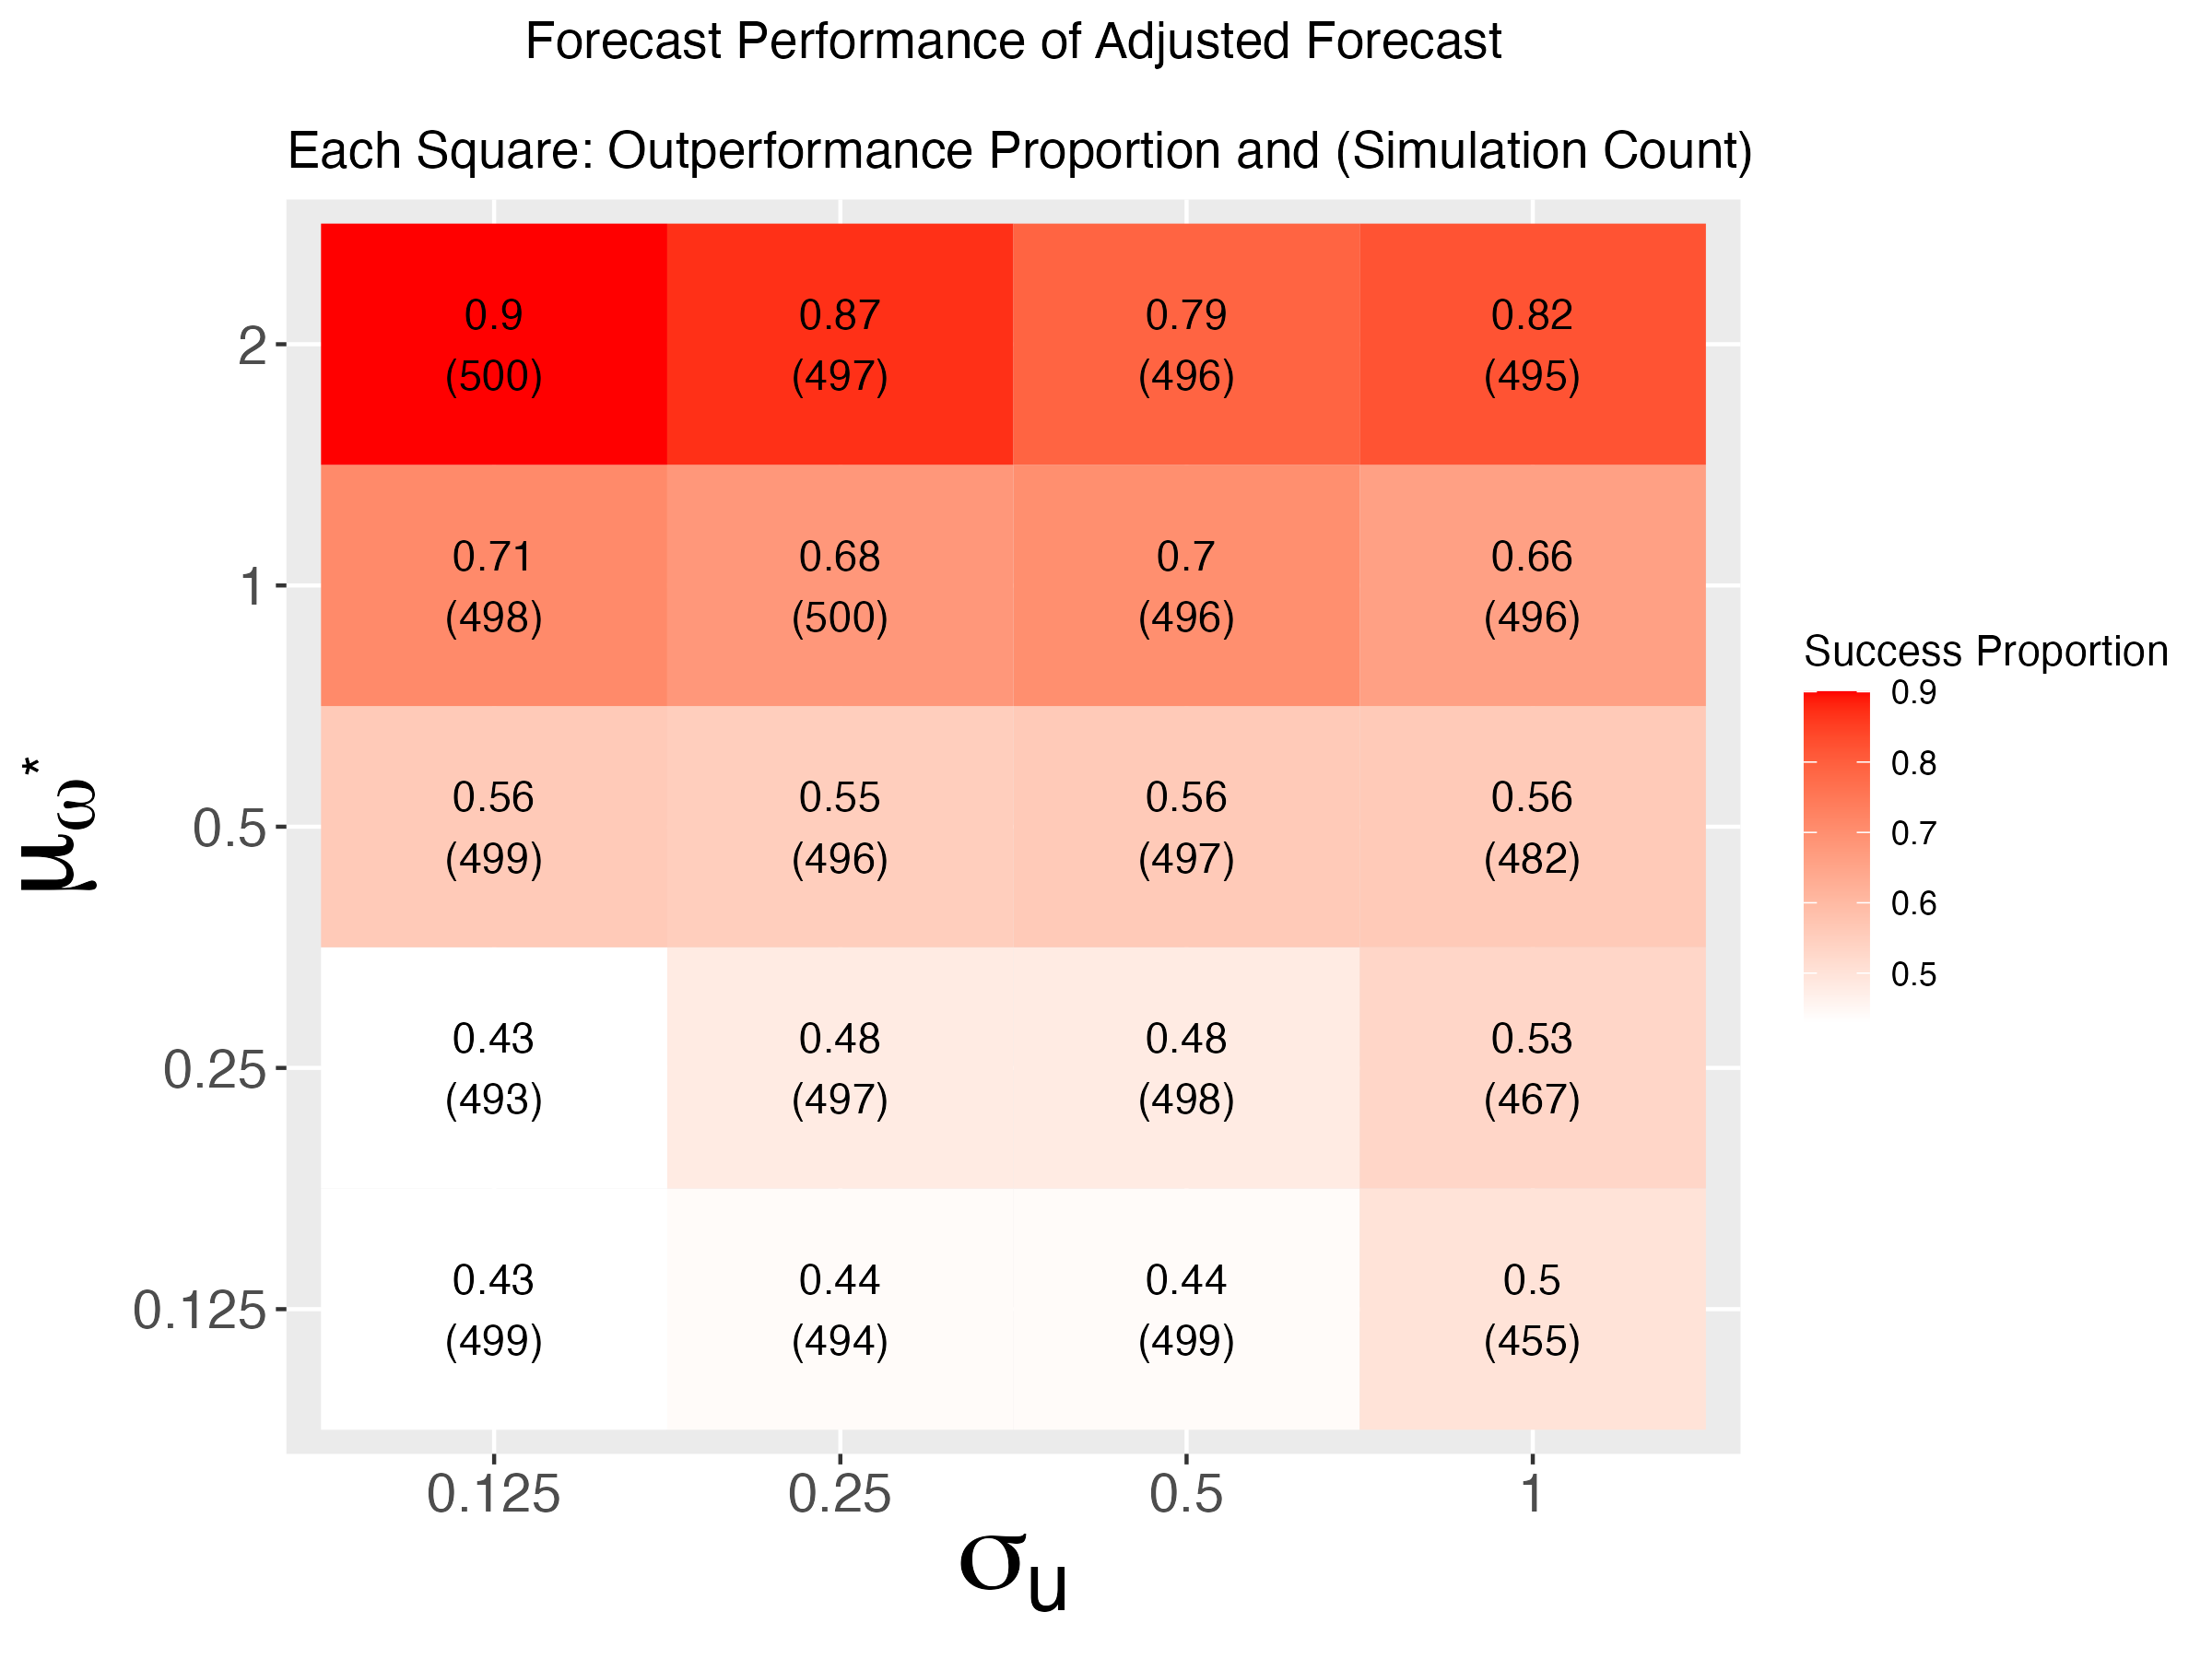
\includegraphics[scale = .42]{simulation_plots/Aug28_224451_2024_mu[omega^*]_sigma[u].png}
% 	  \caption{Fixed values: $\mu_{v} = .125, \sigma_{v} = .125, \delta = .125$}\label{fig:sim_6}
%   \end{subfigure}\hspace{12mm} %
%   \begin{subfigure}{.44\linewidth} 
% 	\centering
% 	  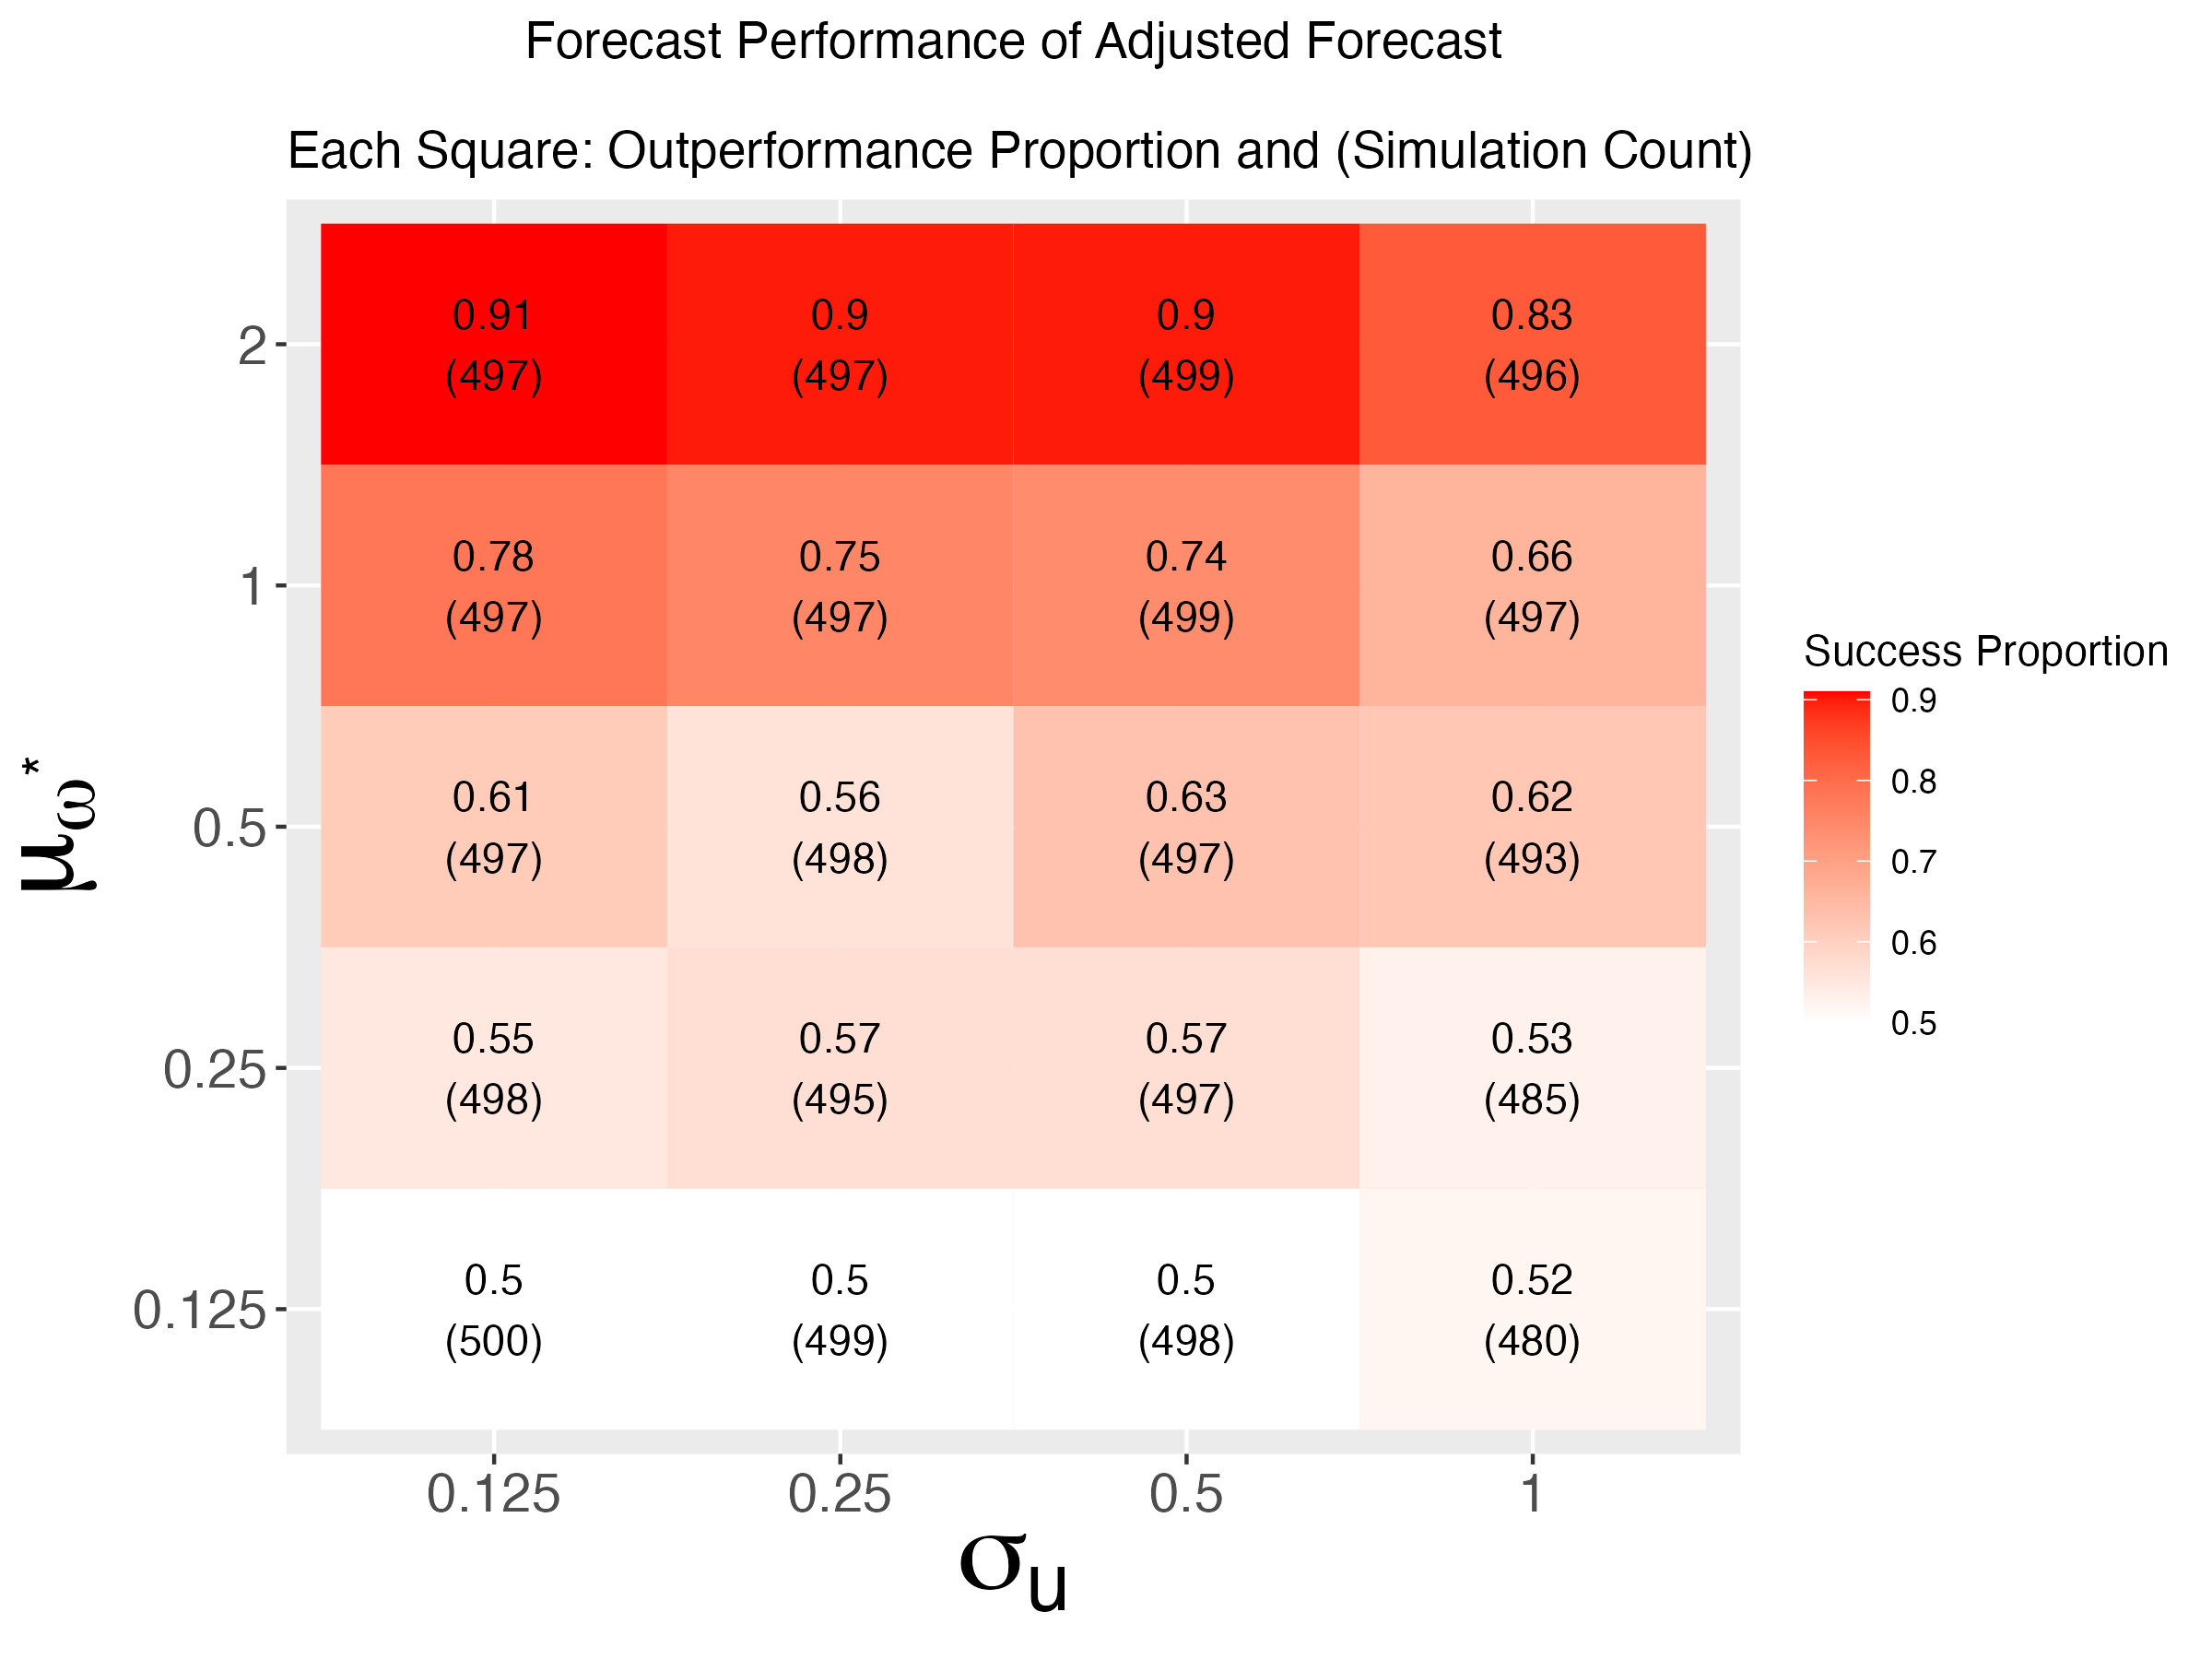
\includegraphics[scale=.42]{simulation_plots/Aug28_224455_2024_mu[omega^*]_sigma[u].png}
% 	  \caption{Fixed values: $\mu_{v} = .125, \sigma_{v} = .125, \delta = 2$}\label{fig:sim_7}
%   \end{subfigure}
  
% 	  \caption{The interaction between the intercept $\mu_{\omega^{*}}$ and $\sigma_{u}$ suggests that the parameters behave as expected.  However, a larger value of $\delta$ in \ref{fig:sim_7} attenuates the effect of increasing noise.}
% 	  \label{fig:intercept_noise}
% 	\end{figure}
%------------------------------------------------

\begin{block}{Real Data Example: Aftermath of Donald Trump's 2016 Victory}
	\begin{figure}
		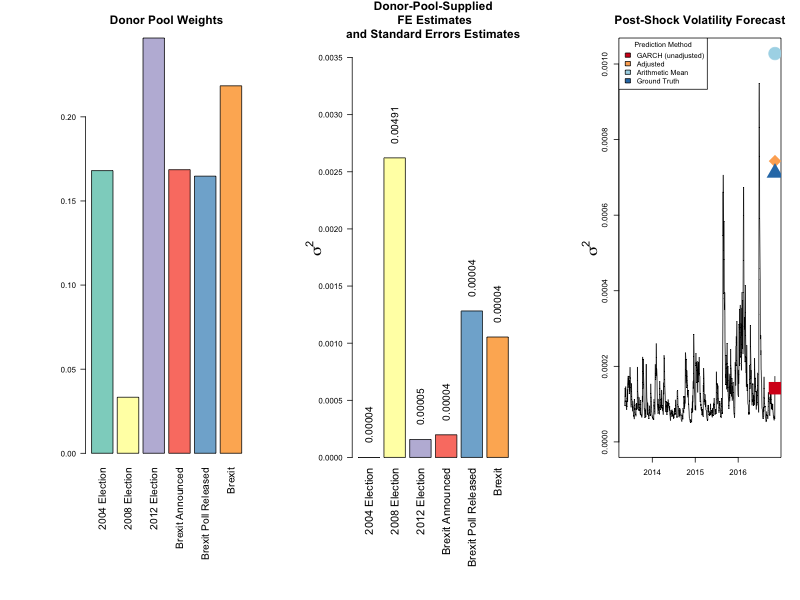
\includegraphics[width=\linewidth]{../real_data_output_plots/WedSep182237432024_IYG_None_None.png}
		\caption{Donor pool weights (left panel), individual shock effects (center panel), and forecasts (right panel).  In the right panel, we predict the volatility of the financial services exchange-traded fund IYG on November 9th, 2016.  The adjusted prediction nearly recovers the realized volatility, which is consistently estimated using high-frequency data.} 
	\end{figure}
\end{block}

%----------------------------------------------------------------------------------------
%	CONCLUSIONS
%----------------------------------------------------------------------------------------

\begin{block}{Conclusions}
	\begin{enumerate}
		\item When news shocks undermine the credibility of the default forecasting model, a new method is called for.
		\item Here we have attempted to model news shocks as parameterized by prevailing risk conditions.
		\item We have also proposed an aggregation mechanism that allows the incorporation of past shock information into current forecasts.
		\item Future directions may involve applications to HAR forecasts, VAR-based forecasts of multivariate time series, and impulse response functions.
	\end{enumerate}
\end{block}

%----------------------------------------------------------------------------------------
%	REFERENCES
%----------------------------------------------------------------------------------------

\begin{block}{References}
	 % Insert publications even if they are not cited in the poster
	%\tiny % Reduce font size
	\vspace{-1ex} % Pull up slightly
	\bibliographystyle{unsrt} % Bibliography style
	\bibliography{../synthVolForecast.bib} % Bibliography file
\end{block}

%----------------------------------------------------------------------------------------
%	ACKNOWLEDGEMENTS
%----------------------------------------------------------------------------------------

%----------------------------------------------------------------------------------------
%	CONTACT INFORMATION
%----------------------------------------------------------------------------------------

\setbeamercolor{block title}{fg=orange} % Change the block title color

\begin{block}{Contact Information}
	\begin{itemize}
		\item Web: \href{https://lunddave.github.io}{https://lunddave.github.io}
		\item Email: \href{mailto:davidpatricklundquist@gmail.com}{davidpatricklundquist@gmail.com}
		\item Find our manuscript on \href{https://arxiv.org/abs/2406.08738}{ArXiv} \cite{lundquist2024volatility}
	\end{itemize}
\end{block}

%----------------------------------------------------------------------------------------

\end{column} % End of the second column

\begin{column}{0.02\textwidth}\end{column} % Empty column for horizontal whitespace

\end{columns} % End of all the columns in the poster

\end{frame} % End of the enclosing frame

%----------------------------------------------------------------------------------------

\end{document}
